\chapter{Web app}
Abbiamo sviluppato una applicazione web interattiva che dimostra alcuni dei nostri risultati.

È strutturata in due parti secondo i principi Restful: Il backend utilizza Flask per poter offrire una semplice API attraverso il quale è possibile sfruttare i modelli allenati ed esporne la funzione \texttt{pred\_prob}, in modo da visualizzare in tempo reale il comportamento del classificatore su di un testo personalizzato, non facente parte del dataset iniziale. Il sistema che abbiamo costruito per esporre i modelli fittati è un buon modo di rendere utilizzabile da chiunque, senza dover passare da script, i risultati del nostro progetto. È facilmente estendibile per altri classificatori e parametri.
\par
Il frontend è sviluppato con Vue JS, un framework Javascript per sviluppare applicazioni reattive. Offre un'interfaccia che consuma l'API appena descritta, visualizzando il risultato della computazione.
\par
Per LDA, un'altra pagina nella stessa applicazione raccoglie sei plot interattivi generati da pyLDAvis, permettendo di consularli e mostrando descrizione, codice e titolo di ognuno degli articoli a cui si riferiscono.

\begin{figure}[H]
  \centering
  \captionsetup{margin=1cm}
  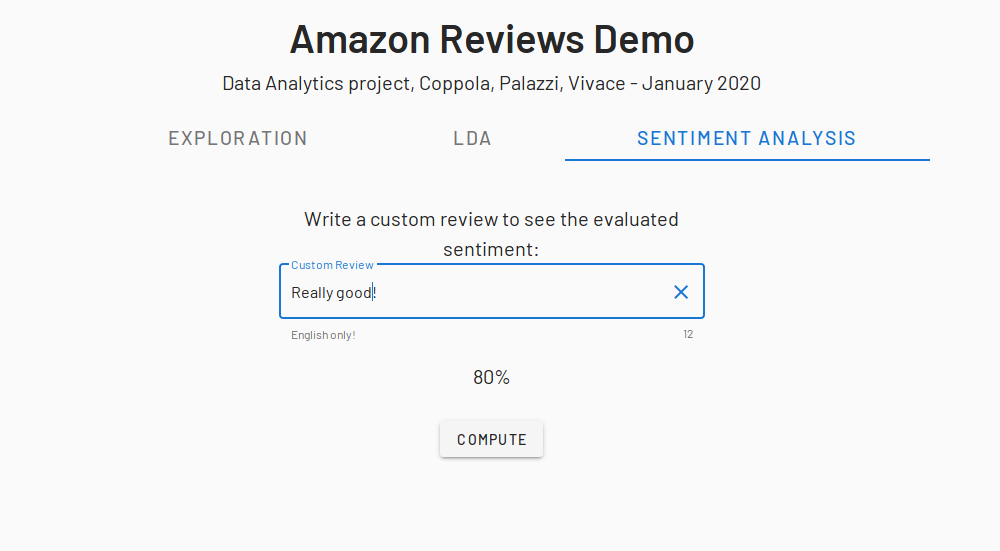
\includegraphics[width=1\linewidth]{figures/ext/webapp1.png}
  \caption{Vista Sentiment Analysis della Demo}
  \label{zipf_law}
\end{figure}

\begin{figure}[H]
  \centering
  \captionsetup{margin=1cm}
  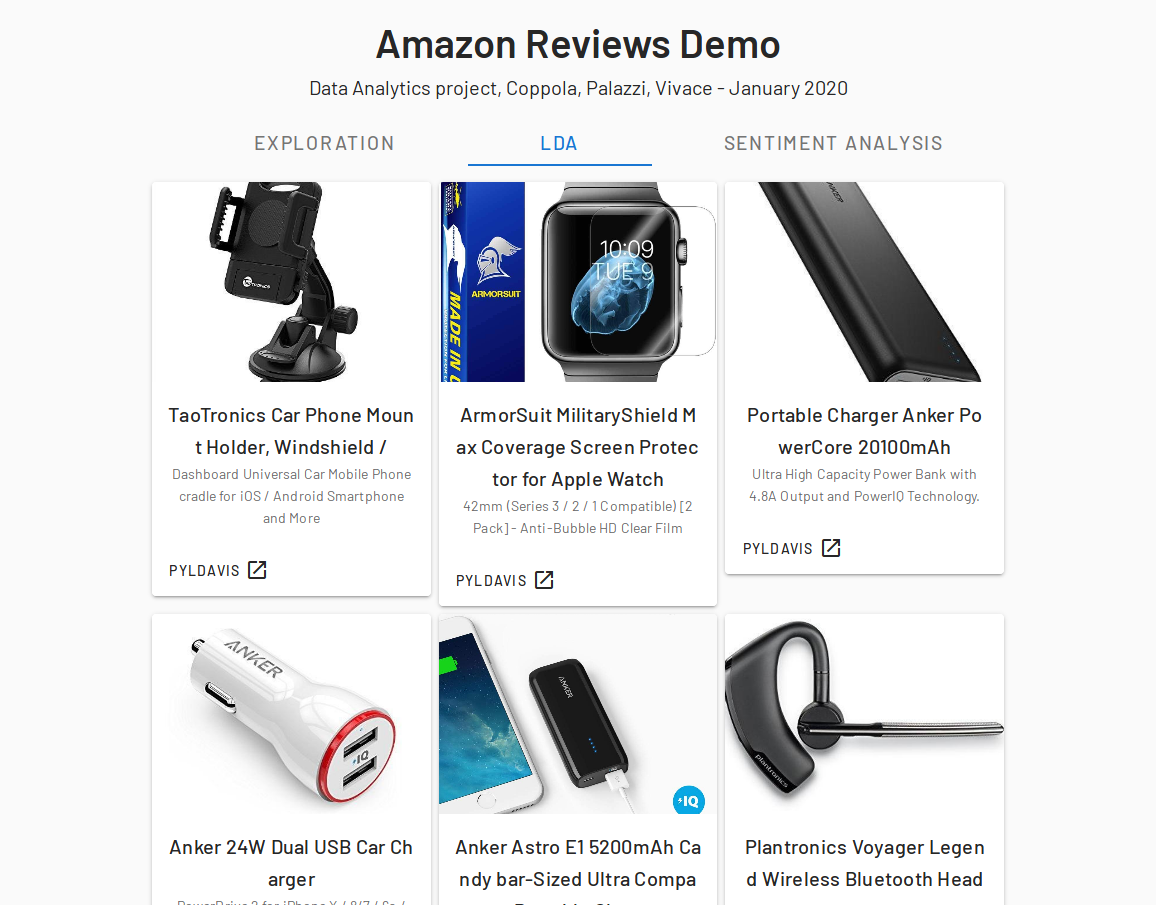
\includegraphics[width=1\linewidth]{figures/ext/webapp2.png}
  \caption{Vista LDA della Demo (pyLDAvis)}
  \label{zipf_law}
\end{figure}

\begin{figure}[H]
  \centering
  \captionsetup{margin=1cm}
  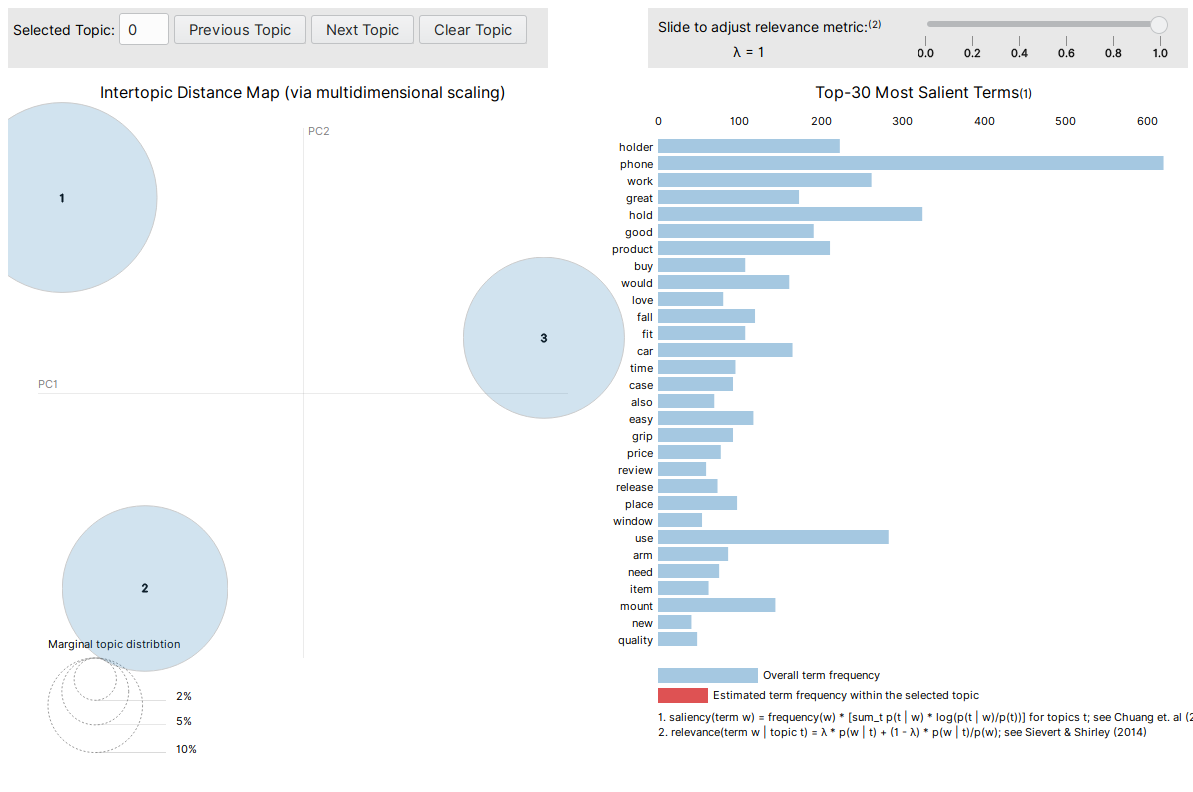
\includegraphics[width=1\linewidth]{figures/ext/webapp3.png}
  \caption{Export pyLDAvis per un singolo prodotto}
  \label{zipf_law}
\end{figure}

\chapter{Conclusioni}
L'esplorazione delle recensioni di prodotti Amazon ci ha permesso di constatare l'enorme numero di informazioni che possono essere estratte da opinioni degli acquirenti con lo scopo di stilare statistiche e valutazioni e poter quindi prendere decisioni in ambito aziendale per migliorare i servizi offerti o centrare meglio la propria clientela.
\par
Lo studio di sentiment analysis dimostra che si possono ottenere modelli addestrati con metriche di controllo molto soddisfacenti e pronti per essere usati nell'analisi sentimentale delle future recensioni.
\par
Per quanto concerne la topic analysis, gli argomenti individuati sui prodotti più recensiti attraverso il modello LDA non sempre sono facili da interpretare. Abbiamo evitato la creazione di argomenti troppo generali ma non abbiamo sempre ottenuto argomenti facilmente utilizzabili per fare ragionamenti complessi sui prodotti. Con ogni probabilità, strumenti più avanzati di topic sentiment analysis porterebbero ad una scelta degli argomenti più logica ed intuitiva.
\par
I modelli utilizzati sono facilmente adattabili a qualsiasi categoria di e-Commerce dotata di una forma di recensioni e, considerati i risultati raggiunti con strumenti base di Data Analytics, non c'è da stupirsi se Amazon sia riuscito a raggiungere la vetta facendo leva su queste tecnologie.